\begin{figure}[h!]
    \centering
    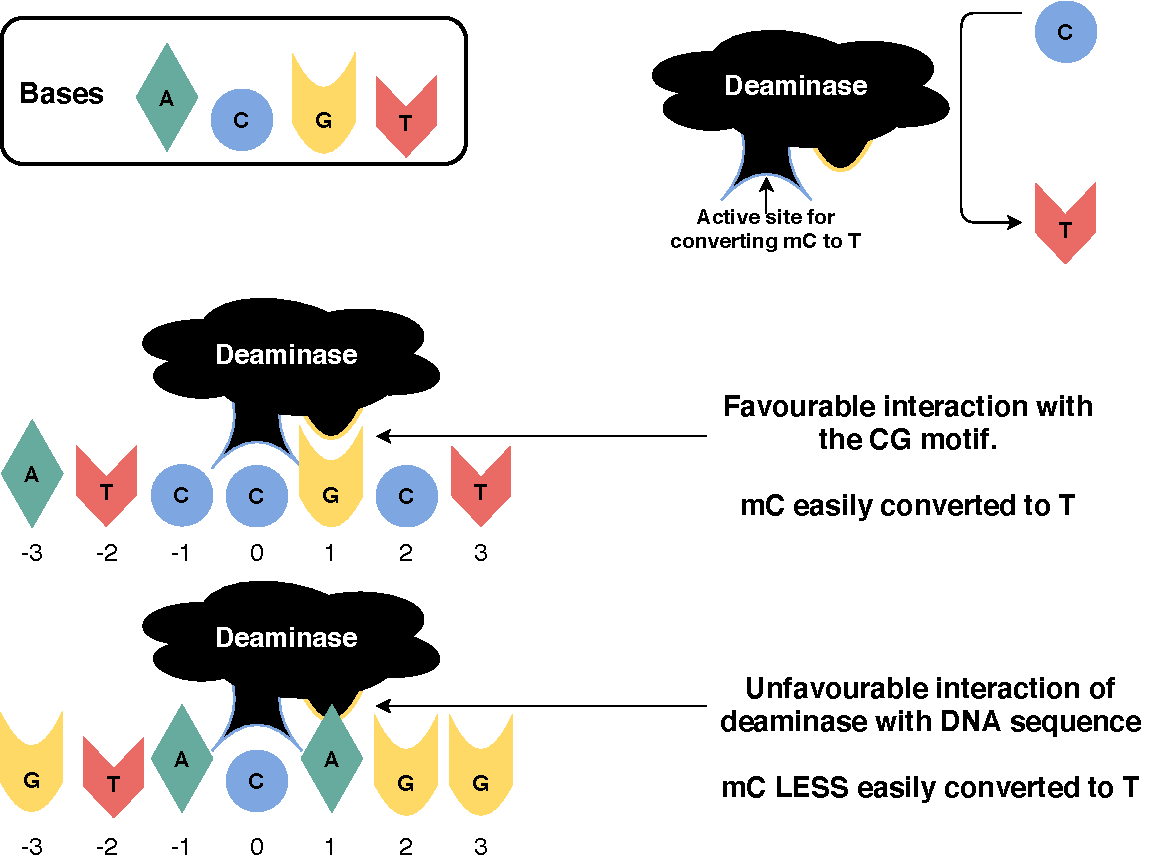
\includegraphics[scale=0.78]{graphics/motif_demo.pdf}
    \caption{\textbf{Mutations are closely linked with the bases next to them}. The schematic diagram depicts an example of hypothetical scenarios that could explain why this is the case. Here, a deaminase protein, which converts methylated C into T, interacts with DNA such that certain sequence contexts make the conversion more feasible than others. While many publications focus on the 3-mer context of mutations (pos -1, 0 and 1), which includes the base change and two bases immediately next to it, evidence shows that bases outside the 3-mer could still be influential. Part of this project seeks to explore the information content available in larger sequence contexts than 3-mers.}
    \label{fig:motif_demo}
\end{figure}
